\documentclass{beamer}

%% Language and font encodings
\usepackage[french]{babel}
\usepackage[utf8x]{inputenc}
\usepackage[T1]{fontenc}

\usetheme{Hannover}
%% Sets page size and margins
%\usepackage[a4paper,top=3cm,bottom=2cm,left=3cm,right=3cm,marginparwidth=1.75cm]{geometry}

%% Useful packages
\usepackage{amsmath,amsfonts,amssymb,amsthm,epsfig,epstopdf,url,array}
\usepackage{graphicx}
\usepackage[colorinlistoftodos]{todonotes}
%\usepackage[colorlinks=true, allcolors=blue]{hyperref}
%\usepackage{comment}
\theoremstyle{plain}
\newtheorem{thm}{Théoreme}[section]
\newtheorem{lem}[thm]{Lemme}
\newtheorem{prop}[thm]{Proposition}
\newtheorem*{cor}{Corollary}
\theoremstyle{definition}
\newtheorem{nota}{Notation}[section]
\newtheorem{defn}{Définition}[section]
\newtheorem{conj}{Conjecture}[section]
\newtheorem{exmp}{Exemple}[section]
%\theoremstyle{proof}
\newtheorem{dem}{Démonstration}
\theoremstyle{remark}
\newtheorem*{rem}{Remark}
%\newtheorem*{note}{Note}

\usepackage{cellspace}
\usepackage{diagbox}

\begin{document}
\title{Le modèle SIR, modélisation des épidémies}
\subtitle{Projet maths-info 2019}
 \author{Marie Bétend - Flore Caye}
 \date{4 Juin 2019}
\begin{frame}
   \maketitle
\end{frame}
\section{Introduction}
\begin{frame}
    \begin{figure}[!h]
\begin{center}
   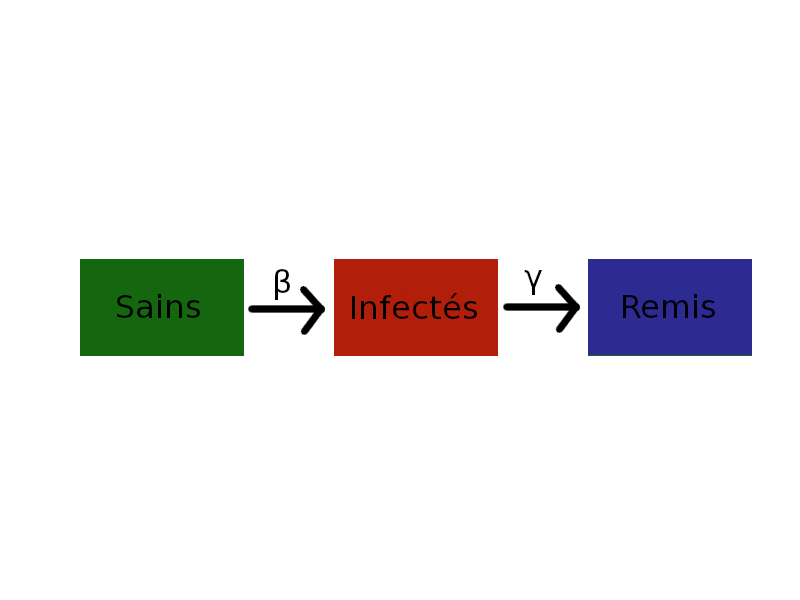
\includegraphics[scale= 1.2]{SIR.png}
   \end{center}
     \caption{Le modèle SIR}
\end{figure}
\end{frame}
\section{Le modèle SIR}
\begin{frame}{Le modèle SIR}
\begin{center}
La population est constante. A tout instant $t > 0$, \\ N = S(t)+I(t)+R(t)
\begin{align}
\label{dS}
&\frac{dS}{dt} = -\beta\frac{SI}{N} \\
\label{dI}
&\frac{dI}{dt} = \beta\frac{SI}{N} - \gamma I \\
\label{dR}  
&\frac{dR}{dt} = \gamma I 
\end{align}
\end{center}
\end{frame}

\begin{frame}{}

\begin{center}
$S(t+\Delta t) = S(t) + C(t + \Delta t)$
\end{center}
et 
\begin{center}
$C(t, \Delta t) \approx \alpha P_{SI}(t, \Delta t)$
\end{center}
\end{frame}
\begin{frame}

    \begin{figure}[!h]
\begin{center}
   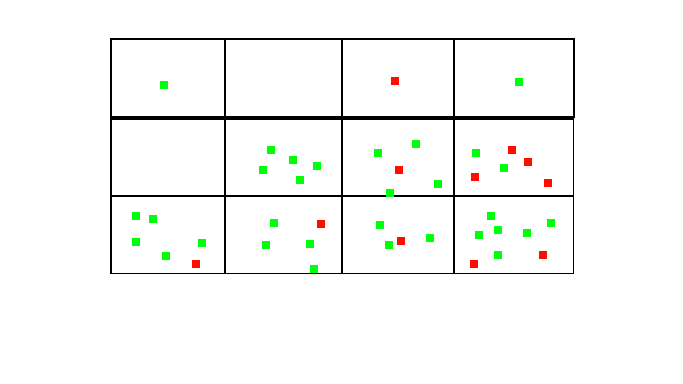
\includegraphics[scale= 0.4]{decoupage.png}
   \end{center}
\end{figure}
P(individu sain se trouve dans une case) = $\frac{S}{M}$ \\
P(un individu infécté se trouve dans une case) =$\frac{I}{M}$\\
Ces deux variables suivent des lois binomiales, de paramètres \\ (S , $\frac{1}{M}$) et (I , $\frac{1}{M}$). Elles sont indépendantes.

\end{frame}

\begin{frame}{Probabilités}
    \begin{align*}
P_{SI}(t, \Delta t) &= P(\text{"il y a au moins un individu sain et un individu infecté sur une case"})\Delta t \\
&=[1 - [P(\text{"il n'y a pas d'individu sain sur une case"}) \\
&(\text{"il n'y a pas d'individus infectés sur une case"})\\
&  - P(\text {"il n'y a pas d'individu sain sur une case"} \cap \\
&\text{"il n'y a pas d'individus infectés sur une case"}]]\Delta t \\
&=[1 - [(1 - \frac{1}{M})^S + (1 - \frac{1}{M})^I \\
&- (1 - \frac{1}{M})^S(1 - \frac{1}{M})^I]]\Delta t \\
\end{align*}
\end{frame}
\begin{frame}
\begin{align*}
P_{SI}(t, \Delta t) &=[1 - [\sum_{k=0}^{S} \binom{S}{k}1^k (\frac{-1}{M})^{S-k}  \\
& + \sum_{k=0}^{I} \binom{I}{k}1^k (\frac{-1}{M})^{I-k} \\
&- \sum_{k=0}^{S} \binom{S}{k}1^k (\frac{-1}{M})^{S-k}\sum_{k=0}^{I} \binom{I}{k}1^k (\frac{-1}{M})^{I-k}]]\Delta t \\
&= [1 - [\sum_{k=0}^{S} \frac{S!}{k!(S-k)!} (\frac{-1}{M})^{S-k}  \\
&+ \sum_{k=0}^{I} \frac{I!}{k!(I-k)!} (\frac{-1}{M})^{I-k} \\
&- \sum_{k=0}^{S} \frac{S!}{k!(S-k)!} (\frac{-1}{M})^{S-k}\sum_{k=0}^{I} \frac{I!}{k!(I-k)!} (\frac{-1}{M})^{I-k}]]\Delta t 
\end{align*}
    
\end{frame}
\begin{frame}{Probabilités}
Pour M suffisamment grand, on a le développement à l'ordre 2 suivant :
\begin{align*}
P_{SI}(t, \Delta t) &=[1 - [1 + \frac{-S}{M}+\frac{S^2-S}{2M^2}+1+\frac{-I}{M}+\frac{I^2-I}{2M^2}- \\
&(1+\frac{-S}{M}+\frac{S^2-S}{2M^2})(1+\frac{-I}{M}+\frac{I^2-I}{2M^2})]]\Delta t \\
&= [1 - 1 + \frac{S}{M} - \frac{S^2-S}{2M^2} - 1+\frac{I}{M} \\
&- \frac{I^2-I}{2M^2} +1+\frac{-I}{M}+\frac{I^2-I}{2M^2} +\frac{-S}{M} \\
&+ \frac{SI}{M^2}+\frac{S^2-S}{2M^2} + o((\frac{-1}{M})^3)]\Delta t \\
&=[\frac{SI}{M^2} +o((\frac{-1}{M})^3)] \Delta t\\
\end{align*}
\end{frame}{}


\begin{frame}
\begin{center}
    $C(t, \Delta t) \approx \alpha SIk \Delta t +  o(\Delta t)$
\end{center}
On pose $\alpha k = \frac{- \beta}{N}$ et on obtient : 
\begin{center}
    $S(t+\Delta t) = S(t) + \frac{- \beta}{N}SI\Delta t + o(\Delta t)$
\end{center}
En supposant que $S$ est une fonction régulière, on a le développement de Taylor suivant :
\begin{align*}
    &S(t + \Delta t) =  S(t) + \Delta t  S^{'}(t)+o(\Delta t)\\
    \Leftrightarrow &S(t) + \Delta t S^{'}(t) + o(\Delta t)= S(t) + \frac{- \beta}{N}SI\Delta t + o(\Delta t)\\
    \Leftrightarrow &S^{'}(t) = \frac{- \beta}{N}SI + o(1)\\
    \Leftrightarrow &S^{'}(t) = \frac{- \beta}{N}SI 
\end{align*}
    

\end{frame}

\begin{frame}
\begin{equation*}
\left\{
\begin{aligned}
S'(t)&= -\beta\frac{S(t)I(t)}{N} \\
I'(t)&= \beta\frac{S(t)I(t)}{N} - \gamma I(t) \\
R'(t)&= \gamma I(t)
\end{aligned}
 \right.
\end{equation*}
\end{frame}
\begin{frame}
\begin{equation*}
\left\{
\begin{aligned}
s'(t)&= -\beta s(t)i(t)\\
i'(t)&= \beta s(t)i(t) - \gamma i(t) \\
r'(t)&= \gamma i(t)
\end{aligned}
 \right.
\end{equation*}
\end{frame}

\begin{frame}{Unicité de la solution}
\begin{align*}
    f: \mathbb{R⁺}\times \mathbb{R^+}\times\mathbb{R^+}\longmapsto \mathbb{R^+}\times\mathbb{R^+}
\end{align*}
\begin{equation*}
    f\left(t,\begin{pmatrix}
    s'(t)\\
    i'(t)\\
    \end{pmatrix}\right)=\begin{pmatrix}- \beta s(t) i(t)\\ \beta s(t) i(t) - \gamma i(t)\\\end{pmatrix}
    \end{equation*}
    \newline
    \newline
    Par le théorème de Cauchy-Lipschitz, il existe une unique solution $\begin{pmatrix}
    s(t)\\
    i(t)\\
    \end{pmatrix}$ sur $\mathbb{R^+}$.
\end{frame}
\begin{frame}{Allure des solutions}
    \begin{itemize}
        \item $s'\leq 0$ donc $s$ est décroissante
        \item $i'=0$ quand $s=\frac{\gamma}{\beta}$, croissant avant, décroissant après 
    \end{itemize}
    \begin{figure}[h]
    \begin{minipage}[c]{.46\linewidth}
        \centering
        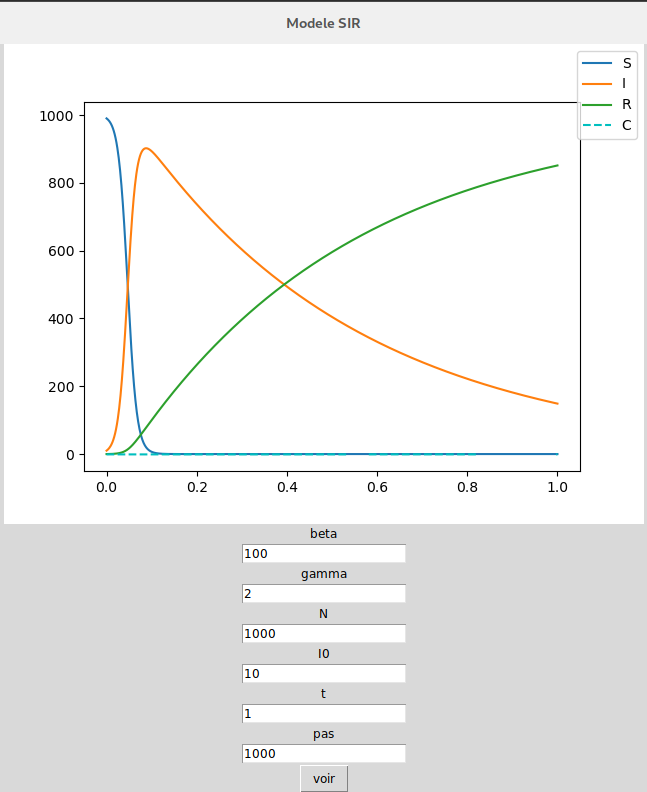
\includegraphics{forte_ep.png}
        \caption{Une forte épidémie}
        \end{minipage}
\end{figure}
\end{frame}
\begin{frame}{Explicitation}
But: trouver une expression de $s$ et fonction de $i$:
\begin{equation*}
\left\{
     \begin{aligned}
    \frac{\mathrm{d}s}{\mathrm{d}t} &= -\beta si\\
    \frac{\mathrm{d}i}{\mathrm{d}t} &= \beta si -\gamma i\\
    \end{aligned}
\right.
\Longrightarrow
\left\{
    \begin{aligned}
    \mathrm{d}s &= -\beta si \mathrm{d}t\\
    \mathrm{d}i &= \left(\beta si -\gamma i \right)\mathrm{d}t\\
    \end{aligned}
    \right.
    \end{equation*}
    \newline
    \begin{equation*}

    \begin{aligned}
    \frac{\mathrm{d}s}{\mathrm{d}i} = \frac{-\beta s}{\beta s-\gamma} \\
    \end{aligned}
    \Longrightarrow
    \begin{aligned}
    \frac{\beta s-\gamma}{-\beta s}\mathrm{d}s=\mathrm{d}i
        \end{aligned}\\
  \text{ en intégrant, on trouve:}
    \begin{aligned}
   \int_{s_0}^{s(t)} \frac{\beta s-\gamma}{-\beta s} \, \mathrm{d}s&=\int_{i_0}^{i(t)}\, \mathrm{d}i \\
   \end{aligned}
 
   \end{equation*}
   \end{frame}
   \begin{frame}
   \begin{equation*}
         \begin{aligned}
    \int_{s_0}^{s(t)} -1+\frac{\gamma}{\beta}\frac{1}{s}\, \mathrm{d}s&=i(t)-i_0\\
        -s(t)+s_0+\frac{\gamma}{\beta}ln(\frac{s(t)}{s_0})&=i(t)-i_0\\
    i(t)+s(t)-\frac{\gamma}{\beta}ln(s(t))&=s_0+i_0-\frac{\gamma}{\beta}ln(s_0)
   \end{aligned}
   \end{equation*}
   On a trouvé une relation explicite entre $s$ et $i$, notons $c(t)=i(t)+s(t)-\frac{\gamma}{\beta}ln(s(t))$. $c(t)$ est une constante pour $t\in\left[0,+\infty\right[$. \\
   
\end{frame}

\begin{frame}{Comparaison modèle et données}
\begin{figure}
    \centering
    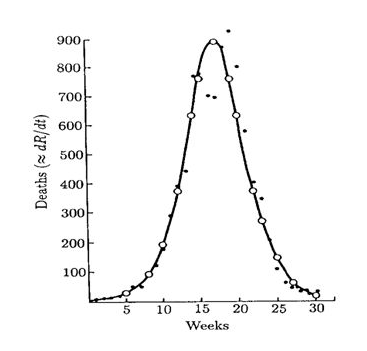
\includegraphics[scale=0.7]{bombay.png}
    \caption{Epidémie de peste de Bombay 1905-1906}
    \label{fig:my_label}
\end{figure}{}
    
\end{frame}{}
\section{Déplacement de population sur un graphe}
\begin{frame}{Déplacement de population sur un graphe}
 \begin{figure}
     \centering
     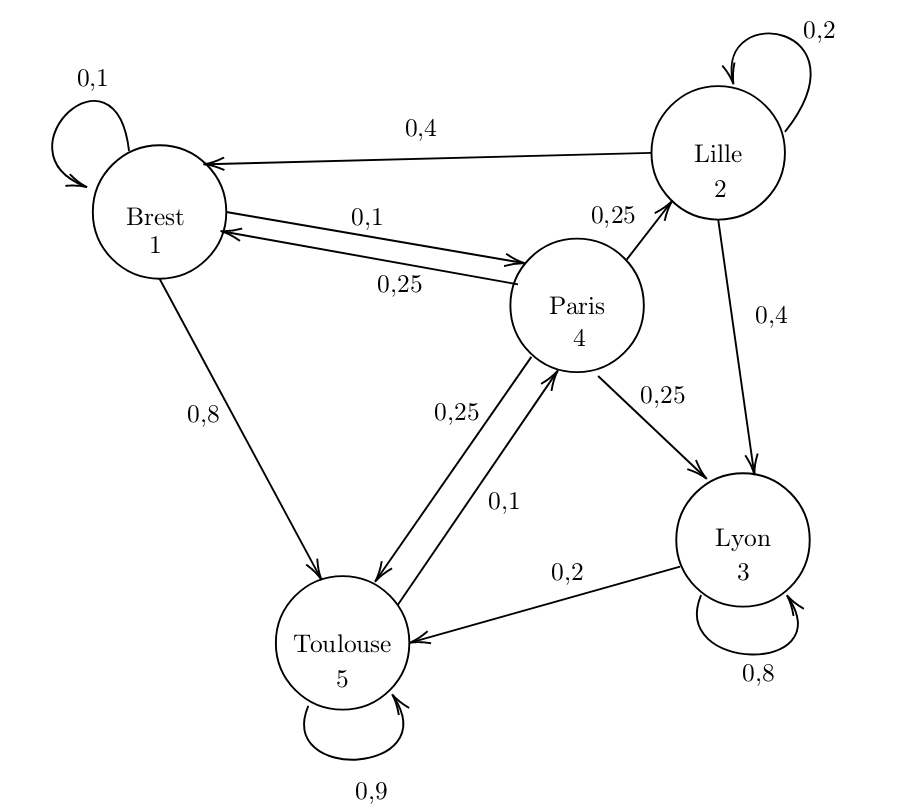
\includegraphics[scale=0.9]{graphe.png}
     \caption{Un exemple de réseau de transport}
 \end{figure}{}
\end{frame}

\begin{frame}{}
En considérant le fait d'être dans une ville comme un état, on peut construire la matrice de transition suivante
$$
V=\begin{pmatrix}
0,1 &0& 0& 0,1 & 0,8\\
0,4 &0,2& 0,4& 0 & 0\\
0 &0& 0,8& 0 & 0,2\\
0,25 &0,25& 0,25& 0 & 0,25\\
0 &0& 0& 0,1 & 0,9
\end{pmatrix}
$$
\end{frame}{}
\begin{frame}{Introduction de la notion de temps}
    ${T(n), n\in\mathbb{N}}$ la séquence des temps de séjour\\
     $T_i(n)$ représente le temps qu'on reste dans une ville $i$ après la $n^{ieme}$ transition.\\
     $$T_i\sim exp(\nu_i)$$
   
\end{frame}
\begin{frame}{Position et transition}
      $$\vec{\pi}(t)=\begin{bmatrix}
\pi_0(t)&...&\pi_r(t)
\end{bmatrix} $$
et $$p_i^j(t)$$ la probabilité de passer de $i$ à $j$ au temps $t$

\end{frame}
\begin{frame}{Pour un petit $\Delta t$}
   $Q$, une matrice de transition de coefficients $q_i^j$.\\
Pour $i\neq j$,\\

\begin{align*}
p_i^j(\Delta t)&=\mathbb{P}(X(\Delta t)=j|X(0)=i) \\
&=\mathbb{P}(T_i(0)\leqslant\Delta t)q_i^j\mathbb{P}(T_j(1)>\Delta t)\\
&=q_i^j\nu_i\Delta t+o(\Delta t)
\end{align*}
Pour $i=j$,\\
\begin{align*}
p_i^i(\Delta t)&=\mathbb{P}(X(\Delta t)=i|X(0)=i)\\
&=\mathbb{P}(T_i(0)>\Delta t)\\
&\approx 1-\nu_i\Delta t+o(\Delta t)
\end{align*}
\end{frame}
\begin{frame}{Equation de Kolmogorov}
    \begin{align*}
\pi_i(t_1+t_2)&=\mathbb{P}(X(t_1+t_2)=i)\\
&=\sum_{j\in E}p_k^i(t_1+t_2)\\
&=\sum_{j\in E}\sum_{k\in E}p_k^i(t_2)p_j^k(t_1)\\
&=\sum_{j\in E}\pi_j(t_1)p_k^i(t_2)
\end{align*}
\end{frame}
\begin{frame}
    \begin{align*}
\pi_i(t+\Delta t)&=\sum_{k\in E}\pi_k(t)p_k^i(\Delta t)\\
&=\sum_{k\in E,k\neq i}\pi_k(t)p_k^i(\Delta t)+\pi_i(t)p_i^i(\Delta t)\\
&=\sum_{k\in E,k\neq i}\pi_k(t)(\nu_i q_k^i\Delta t+o(\Delta t))\\&+\pi_i(t)(1-\nu_i\Delta t+o(\Delta t))\\
&=\sum_{k\in E,k\neq i}\pi_k(t)\nu_iq_k^i\Delta t +\pi_i(t)-\pi_i(t)\nu_i\Delta t + o(\Delta t)
\end{align*}
\end{frame}
\begin{frame}{Un système dynamique}
   $$ \frac{\mathrm{d}\pi_i}{\mathrm{d}t}(t)=\sum_{k\in E,k\neq i}\pi_k(t)q_k^i-\pi_i(t)\nu_i$$
   On reconnait un produit matriciel:
   $$\vec{\pi}'(t)=\vec{\pi}(t)M$$
   Avec
   $$M=
\begin{pmatrix}
-\nu_1 & \nu_1q_1^2&\hdots&\nu_1q_1^r\\
\nu_2q_2^1& -\nu_2&\hdots&\nu_2q_2^r\\
&&\ddots\\
\nu_rq_r^1&\nu_rq_r^2&\hdots&-\nu_r\\
\end{pmatrix}
$$
\end{frame}
\begin{frame}{Etude du système dynamique autonome}
    $$\vec{\pi}'^T(t)=M^T\vec{\pi}^T(t)$$
    Unique solution:
  $$\vec{\pi}(t)=e^{tM^T}\vec{\pi}(0)$$
\end{frame}
\begin{frame}{Propriétés de la matrice M}
    \begin{itemize}
        \item Somme sur les lignes nulle donc population constante
        \item $M\sim Q-I$ donc $\mathrm{R}e(\lambda)\leqslant0$
        \item $m_M(0)=m_Q(1)$, c'est le nombre de composantes connexes 
    \end{itemize}
    De ces propriétés, on déduis la convergence de la solution vers 
    \begin{align*}
\lim\limits_{t \rightarrow +\infty}\vec{\pi}(t)&=P\lim\limits_{t \rightarrow +\infty}\begin{pmatrix}
e^{tJ_{\lambda_1}}&0&\hdots&0\\
0&e^{tJ_{\lambda_2}}&\hdots&0\\
\vdots&\ddots&\ddots&\vdots\\
0&\hdots&0&e^{tJ_{\lambda_i}}\\
\end{pmatrix}P^{-1}\pi(0)\\
\\
&=P\begin{pmatrix}
1&0&\hdots&0\\
0&0&\hdots&0\\
\vdots&\ddots&\ddots&\vdots\\
0&\hdots&0&0\\
\end{pmatrix}P^{-1}\pi(0)\\
\end{align*}
\end{frame}
\section{Fusion des modèles}
\begin{frame}{Fusion des modèles}
    Si les villes ne sont pas reliées entre elles :
    \begin{align*}
    \frac{\mathrm{d}S_i}{\mathrm{d}t}(t)&=-\frac{\beta}{N} S_i(t)I_i(t)\\
    \frac{\mathrm{d}I_i}{\mathrm{d}t}(t)&=\frac{\beta}{N} S_i(t)I_i(t)-\gamma I_i(t)\\
    \frac{\mathrm{d}R_i}{\mathrm{d}t}(t)&=\gamma I_i(t)
\end{align*}
Les vecteurs sont donc de la forme:
\begin{align*}
    \vec{S'}(t)&=-\frac{\beta}{N} \vec{S}(t)\circ\vec{I}(t)\\
   \vec{I'}(t)&=\frac{\beta}{N} \vec{S}(t)\circ\vec{I}(t)-\gamma \vec{I}(t)\\
    \vec{R'}(t)&=\gamma \vec{I}(t)
\end{align*}
\end{frame}{}
\begin{frame}{}
Si les villes sont reliées, on a  $$\vec{\pi'}(t)=\vec{\pi}(t)M$$
On veut prendre en compte :
\begin{itemize}
    \item La population nouvellement arrivée/partie\\
    \item Les transmissions et rémissions de la population, liées à l'évolution de l'épidémie\\
\end{itemize}
D'où
\begin{align*}
    \vec{S'}(t)&=d_S\vec{S}(t)M- \frac{\beta}{N} \vec{S}(t)\circ\vec{I}(t)\\
   \vec{I'}(t)&=d_I\vec{I}(t)M+\frac{\beta}{N} \vec{S}(t)\circ\vec{I}(t)-\gamma \vec{I}(t)\\
    \vec{R'}(t)&=d_R\vec{R}(t)M+\gamma \vec{I}(t)
\end{align*}
\end{frame}

\begin{frame}{Méthodes numériques}
Méthode d'Euler : \\
On cherche une solution pour $y'(t)=f(y(t))$.\\
Elle est donnée par
\begin{align*}
    y(t_0)&=y_0\\
    y(t_{n+1})&=y(t_n)+(t_{n+1}-t_n)f(y(t_n))
\end{align*}
\end{frame}{}
\begin{frame}{Méthodes numériques}
    Méthode du point milieu : \\
    La solution est donnée par 
$$y_{n+1} = y_n + h f \left(y_n + \frac{h}{2} f \left( t, y_n \right) \right)$$
\end{frame}{}
\begin{frame}{Méthodes numériques}
    Méthode de Runge-Kutta d'ordre 4 : \\
    La solution est donnée par
 $$y_{n+1}= y_n+\frac{h}{6}(k_1+2k_2+2k_3+k_4)$$
où \begin{align*}
    k_1&=f(t_n,y_n)\\
    k_2&=f(t_n+\frac{h}{2},y_n+\frac{h}{2}k_1)\\
    k_3&=f(t_n+\frac{h}{2},y_n+\frac{h}{2}k_2)\\
    k4_&=f(t_n+h,y_n+h k_3)
\end{align*}
\end{frame}{}
\begin{frame}{}
    Merci pour votre attention !
\end{frame}{}
\section{Bibliographie}
\begin{frame}{Bibliographie}

\href{http://www.fields.utoronto.ca/video-archive/static/2018/03/2365-18260/mergedvideo.ogv}{Uncovering the epidemic pattern of medieval plagues}

\href{http://marcchoisy.free.fr/pdf/DeBoeck2010.pdf}{Modélisation mathématique en épidémiologie}


\href{https://docplayer.fr/365545-Module-7-chaines-de-markov-a-temps-continu.html}{Chaînes de Markov, cours, EPFL, Patrick Thiran}
\bibitem{}
    J.D. Murray,
  \textit{Mathematical Biology},
  I : An Introduction, Springer,
  3nd edition
\end{frame}{}
\end{document}